\hypertarget{Human_8cpp}{}\section{app/\+Human.cpp File Reference}
\label{Human_8cpp}\index{app/\+Human.\+cpp@{app/\+Human.\+cpp}}


The file \hyperlink{Human_8cpp}{Human.\+cpp} implements the \hyperlink{classHuman}{Human} class. The class will be used in \hyperlink{classXingyun}{Xingyun} class.  This project is released under the B\+S\+D-\/3-\/\+Clause License.  


{\ttfamily \#include $<$iostream$>$}\\*
{\ttfamily \#include $<$vector$>$}\\*
{\ttfamily \#include $<$Human.\+hpp$>$}\\*
Include dependency graph for Human.\+cpp\+:
\nopagebreak
\begin{figure}[H]
\begin{center}
\leavevmode
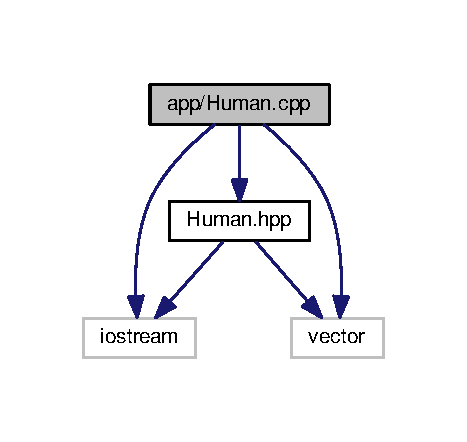
\includegraphics[width=224pt]{Human_8cpp__incl}
\end{center}
\end{figure}


\subsection{Detailed Description}
The file \hyperlink{Human_8cpp}{Human.\+cpp} implements the \hyperlink{classHuman}{Human} class. The class will be used in \hyperlink{classXingyun}{Xingyun} class.  This project is released under the B\+S\+D-\/3-\/\+Clause License. 

Copyright (c) 2019 Hao Da (Kevin) Dong, Zuyang Cao, Jing Liang

\begin{DoxyDate}{Date}
10/13/2019 
\end{DoxyDate}
